\documentclass[11pt]{article}
\usepackage[a4paper,margin=21mm]{geometry}
\usepackage{fontspec,xeCJK}
\setmainfont{DejaVu Serif}
\setmonofont{DejaVu Sans Mono}[Scale=.78]
\setCJKmainfont[AutoFakeBold=2,AutoFakeSlant=.15]{Droid Sans Fallback}
\setCJKmonofont{Droid Sans Fallback}
\xeCJKDeclareCharClass{Default}{"201C,"201D}
\usepackage{amsmath,amssymb,bm,booktabs,array}
\usepackage{xcolor,graphicx,tikz,fancyvrb}
\usepackage{float}
\usetikzlibrary{arrows.meta,positioning,calc,fit,backgrounds}
\usepackage[colorlinks=true,linkcolor=blue!55!black,urlcolor=blue!55!black]{hyperref}
\setlength{\parskip}{.45em}
\setlength{\emergencystretch}{3em}
\setlength{\parindent}{0pt}
\renewcommand{\figurename}{图}
\newcommand{\tS}{\widetilde S}
\newcommand{\ET}{\mathcal E_T}
\newcommand{\EZ}{\mathcal E_0}
\newcolumntype{P}[1]{>{\raggedright\arraybackslash}p{#1}}
\definecolor{rc}{RGB}{215,230,252}
\definecolor{lc}{RGB}{223,241,218}
\definecolor{oc}{RGB}{255,226,191}
\tikzset{r/.style={draw,fill=rc,rounded corners=2pt,minimum width=10mm,minimum height=7mm},
 l/.style={r,fill=lc},o/.style={r,fill=oc,rounded corners=0pt},
 envcap/.style={draw,fill=gray!12,rounded corners=2pt,minimum width=9mm,minimum height=8mm},
 box/.style={draw,rounded corners=3pt,align=center,inner sep=7pt},
 wire/.style={line width=.7pt},arr/.style={-{Stealth[length=2mm]},line width=.8pt},
 hole/.style={draw,dashed,minimum width=15mm,minimum height=8mm,fill=white},
 every node/.style={font=\small}}
\newcommand{\takeaway}[1]{\begin{center}\fcolorbox{blue!40}{blue!3}{\parbox{.93\linewidth}{#1}}\end{center}}
\title{我们到底怎样收缩这个 fPEPS？\\[2mm]\large 从两条边界 MPS 到中心方程和 bare/direct 熵的图解}
\author{PEPS3EE 技术说明}
\date{2026 年 9 月 22 日\quad 图解版 v21}
\begin{document}
\maketitle
\section*{先给出路线，不从运行日志开始}
\takeaway{\textbf{当前路线：用两条独立无限 MPS 表示相反两侧的环境，建立依赖这两条 MPS 的中心残差方程，再用信赖域求根同时更新它们。}\\
方程采用双边中心投影；实际更新是自写残差求根程序。标准 biVUMPS 的逐次中心本征更新、CTMRG 的边角更新，是另外两种更新方法。}

\begin{figure}[h]\centering
\begin{tikzpicture}[node distance=7mm]
\node[box,fill=oc,text width=12cm] (a) {固定输入：exact $D=2$ fPEPS 局域张量 $P$\\物理系统始终无限；改变 $\chi$ 只改变环境近似};
\node[box,fill=rc,text width=12cm,below=of a] (b) {未知量：$|R(A)\rangle$ 和 $\langle L(B)|$ 两条独立无限 MPS\\每条链无限长，每个虚键只保留 $\chi$ 个态};
\node[box,text width=12cm,below=of b] (c) {每轮重建混合环境，计算 site/bond 中心残差\\求出 $\delta A,\delta B$，检验新张量是否真正减小原残差};
\node[box,fill=lc,text width=12cm,below=of c] (d) {环境通过检查后冻结：关联函数、Gaussian 对比、bare/direct $\tS$};
\draw[arr] (a)--(b);\draw[arr] (b)--(c);\draw[arr] (c)--(d);
\draw[arr] (c.east)--++(.45,0)|-(b.east);
\end{tikzpicture}
\caption{主路线只有这四层。初值可以来自其他方法，但初值来源不改变实际更新的未知量。}
\end{figure}

\textbf{当前结果的边界：}小 $\chi$ 有通过中心方程的对照；当前研究的 gapless
$\chi=16$ 尚无通过全部检查的新环境。本文解释实际实现，不把它包装成已经解决收敛问题的算法。

阅读顺序：第 1--5 节回答“收缩什么、解什么、怎样更新”；第 6 节说明费米子符号；
第 7--8 节说明熵与关联长度。尝试记录、具体参数和提交命令放在附录。
旧的 35 页运行记录另存为 \href{appendix_experiments_v18.pdf}{实验记录附册}，不再作为技术正文。
\clearpage

\section{未知量到底是什么？}
设局域 fPEPS 张量为 $P^p_{l r u d}$。物理指标 $p$ 与共轭层收缩后得到双层张量 $O$，
沿一行排列成为行转移 MPO $\mathbb T$。每条复合虚腿包含 ket、bra 两根 $D=2$ 的腿。
全文图例：蓝色是右 MPS，绿色是左 MPS，橙色是固定 PEPS；连线表示收缩，悬空线表示保留指标。
\begin{figure}[h]\centering
\begin{tikzpicture}[x=1cm,y=1cm]
\node[o] (p) at (0,0) {$P$};\node[o] (pb) at (2,0) {$\bar P$};
\draw[wire] (p.north)--++(0,.65)node[above]{$u$};
\draw[wire] (p.south)--++(0,-.65)node[below]{$d$};
\draw[wire] (p.west)--++(-.65,0)node[left]{$l$};
\draw[wire] (p.south east)--++(.45,-.5)node[right]{$r$};
\draw[wire] (pb.north)--++(0,.65);\draw[wire] (pb.south)--++(0,-.65);
\draw[wire] (pb.east)--++(.65,0);\draw[wire] (pb.south west)--++(-.4,-.5);
\draw[wire] (p.east)--node[above]{$p$}(pb.west);
\draw[arr] (3.1,0)--(4.2,0);
\node[o] (O) at (5.3,0) {$O$};
\draw[wire] (O.north)--++(0,.8)node[above]{$s=(u,\bar u)$};
\draw[wire] (O.south)--++(0,-.8)node[below]{$t=(d,\bar d)$};
\draw[wire] (O.west)--++(-.65,0)node[left]{$m$};
\draw[wire] (O.east)--++(.65,0)node[right]{$m'$};
\node[align=left] at (9,0) {$s,t,m,m'$ 的维数为 $D^2$\\交换与 dual 符号见第 6 节};
\end{tikzpicture}
\caption{双层局域张量。图标明连通关系；复合腿的内部次序固定，不能按普通数组随意交换。}
\end{figure}

精确半平面边界满足 $\mathbb T|R\rangle=\lambda|R\rangle$、
$\langle L|\mathbb T=\lambda\langle L|$。
我们把它们近似为两个一站点平移不变 MPS：$|R(A)\rangle$ 和 $|L(B)\rangle$，
后者取 bra 后进入收缩。$A$ 与 $B$ 是独立变量。
\begin{figure}[h]\centering
\begin{tikzpicture}[x=1.65cm,y=.9cm]
\foreach \j in {0,1,2,3}{
\node[r] (a\j) at (\j,1) {$A$};\node[o] (o\j) at (\j,0) {$O$};
\node[l] (b\j) at (\j,-1) {$\bar B$};
\draw[wire] (a\j)--node[right,font=\scriptsize]{$s$}(o\j)--node[right,font=\scriptsize]{$t$}(b\j);}
\foreach \i/\j in {0/1,1/2,2/3}{\foreach \n in {a,o,b}{\draw[wire] (\n\i)--(\n\j);}}
\foreach \n/\y in {a/1,o/0,b/-1}{\draw[dashed] (-.7,\y)--(\n0);\draw[dashed] (\n3)--(3.7,\y);}
\node[right] at (3.8,1) {$|R\rangle$：一条 MPS};
\node[right] at (3.8,0) {$\mathbb T$：固定 PEPS 行};
\node[right] at (3.8,-1) {$\langle L|$：另一条 MPS};
\end{tikzpicture}
\caption{无限条带的收缩，左右虚线延伸到无穷。有限的是 MPS 键维 $\chi$，不是物理系统长度。}
\end{figure}

每条 MPS 都以 mixed canonical form 存储，而不是把整条无限链称作“左规范 MPS”：
\[
\cdots A_L\ A_L\ \boxed{A_C}\ A_R\ A_R\cdots,
\qquad A_C=A_LC_A=C_AA_R.
\]
左侧半无限尾部是左规范 $A_L$，右侧半无限尾部是右规范 $A_R$，中间可用 site-center
$A_C$ 或 bond-center $C_A$ 表示。后文的 $\ell,r$ 表示同一条 MPS 的左右规范，
$R,L$ 则表示两条不同 MPS。

\takeaway{一组方向的求解未知量是两条 MPS。另一空间方向需要对整体旋转后的图另行处理。
本求解器不把四个 CTM 角和四条 CTM 边当作更新变量。}
\clearpage

\subsection{先定义符号：\texorpdfstring{$\rho_A$、$C_A$ 和 $A_C$}{rhoA、CA 和 AC}}
先只看右边界 $|R(A)\rangle$。把 site 张量的复合指标 $s=1,\ldots,d$ 固定后，
$A_\ell^s$ 是 $\chi\times\chi$ 矩阵；本例 $d=D^2=4$。
左 canonical 的意思是 $\sum_s(A_\ell^s)^\dagger A_\ell^s=I$。

\textbf{$\rho_A$：这条 MPS 自己的右转移固定点。}
用 $A_\ell$ 和它\emph{自己的共轭}构造
\[
\mathcal E_A(X)=\sum_s A_\ell^sX(A_\ell^s)^\dagger,
\qquad \boxed{\mathcal E_A(\rho_A)=\rho_A,\quad
\rho_A\ge0,\quad\operatorname{tr}\rho_A=1.}
\]
这里给出有序复合指标下的矩阵写法；实现用带 graded 腿的自转移收缩。
它只使用 $A_\ell$，不使用另一条边界 $B$，也不夹 PEPS 行 $O$。
\begin{figure}[H]\centering
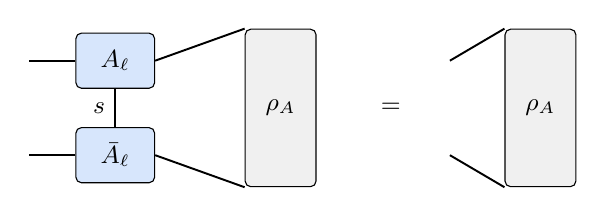
\begin{tikzpicture}[x=1cm,y=.8cm]
\node[r] (a) at (0,.75) {$A_\ell$};\node[r] (b) at (0,-.75) {$\bar A_\ell$};
\node[envcap,minimum height=20mm] (rho) at (2.1,0) {$\rho_A$};
\draw[wire] (a.east)--(rho.north west);\draw[wire] (b.east)--(rho.south west);
\draw[wire] (a)--node[left]{$s$}(b);
\draw[wire] (a.west)--(-1.1,.75);\draw[wire] (b.west)--(-1.1,-.75);
\node at (3.5,0) {$=$};
\node[envcap,minimum height=20mm] (out) at (5.4,0) {$\rho_A$};
\draw[wire] (out.north west)--(4.25,.75);\draw[wire] (out.south west)--(4.25,-.75);
\end{tikzpicture}
\caption{自转移固定点方程：把一对 $A_\ell,\bar A_\ell$ 接到右侧固定点，得到相同的两腿矩阵。}
\end{figure}

\textbf{$C_A$：一条虚键上的中心矩阵，大小为 $\chi\times\chi$。}
把这条 MPS 从一个键切开，在左右正交半链基底中写成
\[
|R\rangle=\sum_{\alpha,\beta}(C_A)_{\alpha\beta}
|\Phi^\ell_\alpha\rangle|\Phi^r_\beta\rangle,
\qquad \rho_A=C_AC_A^\dagger.
\]
$C_A$ 的奇异值是\emph{边界 MPS}的 Schmidt 系数，$\rho_A$ 的本征值是其平方。
一般 $C_A$ 有规范自由；当前代码特意选正中心规范 $C_A=\sqrt{\rho_A}$，没有要求它对角。

\textbf{$A_C$：包含一个 site 的中心张量，有两个虚指标和一个复合指标 $s$。}
\[
\boxed{A_C^s=A_\ell^s C_A=C_AA_r^s,\qquad
A_r^s=C_A^{-1}A_\ell^sC_A.}
\]
\begin{figure}[H]\centering
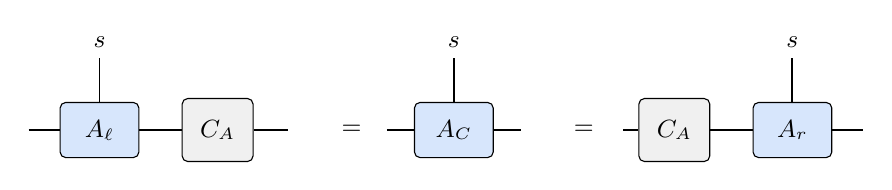
\begin{tikzpicture}[x=1cm,y=.8cm]
\node[r] (a) at (0,0) {$A_\ell$};\node[envcap] (c) at (1.5,0) {$C_A$};
\draw[wire] (-.9,0)--(a);\draw[wire] (a)--(c);\draw[wire] (c)--(2.4,0);
\draw[wire] (a.north)--++(0,.7)node[above]{$s$};
\node at (3.2,0) {$=$};\node[r] (ac) at (4.5,0) {$A_C$};
\draw[wire] (3.65,0)--(ac)--(5.35,0);\draw[wire] (ac.north)--++(0,.7)node[above]{$s$};
\node at (6.15,0) {$=$};\node[envcap] (cr) at (7.3,0) {$C_A$};\node[r] (ar) at (8.8,0) {$A_r$};
\draw[wire] (6.65,0)--(cr)--(ar)--(9.7,0);\draw[wire] (ar.north)--++(0,.7)node[above]{$s$};
\end{tikzpicture}
\caption{$C_A$ 只有两条虚腿；$A_C$ 还带一个 site 指标。它们不是同一个张量。}
\end{figure}
当前保留支撑内要求 $\rho_A$ 满秩，故上式可取逆，并得到 $\sum_s A_r^s(A_r^s)^\dagger=I$。

左边界 $B$ 独立作同样构造，得到 $\rho_B,C_B,B_C,B_r$。
\textbf{下标 $A$ 在这里表示“MPS 张量 $A$ 所属的量”，不是二维物理区域 $A$；
$\rho_A$ 也不是上下两条 MPS 的混合固定点。}
\clearpage

\section{怎样把两条无限 MPS 收成有限环境？}
沿\emph{横向}增加一列，得到两个有限维线性映射：直接重叠 $\EZ$，以及夹 PEPS 行的 $\ET$。
这里的“横向”是 boundary MPS 的传播方向；一列中的纵向对象依次是上边界 MPS、
中间的一层 PEPS 双层张量 $O$、下边界 MPS。因而 $\ET$ 是一个\textbf{三层混合 channel}。
它不是三条 MPS，也不是把三层一次性收成一个数；左右还各留下一个 cap 的开放复合腿。
删掉中间 $O$ 后得到 $\EZ$，只有上下两层 boundary MPS，是 bare overlap channel。
\begin{figure}[h]\centering
\begin{tikzpicture}[x=1cm,y=1cm]
\node[envcap,minimum height=18mm] (x) at (0,0) {$X$};
\node[r] (a) at (1.8,.65) {$A$};\node[l] (b) at (1.8,-.65) {$\bar B$};
\draw[wire] (x.north east)--(a.west);\draw[wire] (x.south east)--(b.west);
\draw[wire] (a)--(b);\draw[wire] (a.east)--(3,.65);\draw[wire] (b.east)--(3,-.65);
\node at (1.4,-1.35) {$\EZ(X)$，两根开放虚腿};
\node[envcap,minimum height=25mm] (y) at (6,0) {$Y$};
\node[r] (c) at (8,1) {$A$};\node[o] (o) at (8,0) {$O$};\node[l] (d) at (8,-1) {$\bar B$};
\draw[wire] (y.north east)--(c.west);\draw[wire] (y.east)--(o.west);\draw[wire] (y.south east)--(d.west);
\draw[wire] (c)--(o)--(d);\foreach \n/\h in {c/1,o/0,d/-1}{\draw[wire] (\n.east)--(9.3,\h);}
\node at (7.8,-1.65) {$\ET(Y)$，三根复合开放虚腿};
\end{tikzpicture}
\caption{一步 transfer 就是把一列接到 cap 上。左图没有 $O$，右图有 $O$；两者都依赖当前的 $A,B$。}
\end{figure}

在指定有向基底中，收缩规则可写为
\begin{align}
[\EZ(X)]_{b'a'}&=\sum_{b,a,s}^{\rm graded}\bar B^s_{bb'}A^s_{aa'}X_{ba},\\
[\ET(Y)]_{b'm'a'}&=\sum_{b,m,a,s,t}^{\rm graded}\bar B^t_{bb'}O^{ts}_{mm'}A^s_{aa'}Y_{bma}.
\end{align}
上标 graded 表示按图中的腿顺序做有符号收缩，具体规则在第 6 节；它不是可忽略的符号。

每个通道各求两端的主固定点：
\[
\ell_0E_0=\mu_0\ell_0,\quad E_0r_0=\mu_0r_0,
\qquad \ell_TE_T=\mu_T\ell_T,\quad E_Tr_T=\mu_Tr_T.
\]
这里的左右作用是相应有向图的线性/对偶作用；实际实现保留 cups 和 twists。
两种 canonical chart 分别提供左端和右端的张量。
具体地，按 mixed gauge，代码中的四个对象是
\[
\begin{array}{c|c|c}
\text{对象}&\text{固定点方程}&\text{图中包含}\\ \hline
\ell_T&\mathcal E_{T,L}(\ell_T)=\mu_T\ell_T
&A_L\;--\;O\;--\;\bar B_L\\
r_T&\mathcal E_{T,R}(r_T)=\mu_T r_T
&A_R\;--\;O\;--\;\bar B_R\\
\ell_0&\mathcal E_{0,L}(\ell_0)=\mu_0\ell_0
&A_L\;--\;\bar B_L\quad(O\text{ 被删去})\\
r_0&\mathcal E_{0,R}(r_0)=\mu_0 r_0
&A_R\;--\;\bar B_R\quad(O\text{ 被删去})
\end{array}
\]
所以 $\ell_T$ 确实是 $A_L$--$O$--$\bar B_L$ channel 的左环境，
$r_T$ 是 $A_R$--$O$--$\bar B_R$ channel 的右环境。
代码中的 $O$ 先经过 \texttt{bv\_grow} 做 graded fusion、dual 和端口重排；
上式是网络层次的记号，不是普通无符号矩阵乘积。它们不同于
$\rho_A,\rho_B$（各自单条 MPS 的自转移固定点），也不同于后面求出的中心张量 $A_C,B_C$。
\begin{figure}[h]\centering
\begin{tikzpicture}
\node[envcap] (l) at (0,0) {$\ell_T$};
\node[box,fill=gray!4,minimum width=65mm] (e) at (4,0) {$\cdots\ E_T\ E_T\ E_T\ \cdots$};
\node[envcap] (r) at (8,0) {$r_T$};
\draw[wire] (l)--(e)--(r);
\node[align=center] at (4,-1) {左右无穷多列 $\longrightarrow$ 两个有限 cap\\$\ell_0,r_0$ 对直接重叠做同样的事};
\end{tikzpicture}
\caption{$\ell_T$ 是 $A_L$--$O$--$\bar B_L$ channel 的左 cap，$r_T$ 是
$A_R$--$O$--$\bar B_R$ channel 的右 cap；$\ell_0,r_0$ 分别是删去 $O$ 后
$A_L$--$\bar B_L$、$A_R$--$\bar B_R$ 的直接重叠 cap。四个 cap 是内层线性固定点问题的解，
两条 boundary MPS 是外层非线性问题的未知量；两者不能混称。}
\end{figure}

\takeaway{本页得到四个 cap 和一个每列行商 $q=\mu_T/\mu_0$。
cap 残差很小，只说明当前 $A,B$ 所定义的通道收好了；它不说明 $A,B$ 已是正确半平面边界。}
\clearpage

\section{把中心挖空，究竟得到什么方程？}
固定本轮 cap 后，把上边界的中心张量记作输入 $a$；下边界中心暂时不放入，
留下它的三个指标作输出。以下虚线框表示\emph{未收缩的输出指标}，不是额外张量。
这里的符号对应代码中的实际对象：
\[
\boxed{a=R.AC[1]=A_C,\qquad c=R.C[1]=C_A,}
\qquad
b=L.AC[1]=B_C,\quad d=L.C[1]=C_B.
\]
$a$ 带一个 site 指标和两个 MPS 虚指标，矢量化后维数为 $d\chi^2$；
$c$ 只有两个虚指标，矢量化后维数为 $\chi^2$。
图里没有画出的下边界输入分别是 $b$ 和 $d$；因此把输出框填上
$\bar b$ 或 $\bar d$ 后，才得到一个标量。$a,c$ 不是物理位置上的两个 site，
也不是任意独立的两个优化变量：它们由同一条右边界的 $A_\ell,C_A,A_r$ 共同决定。
\begin{figure}[h]\centering
\begin{tikzpicture}[x=1cm,y=.9cm]
\node[envcap,minimum height=25mm] (l) at (0,0) {$\ell_T$};
\node[envcap,minimum height=25mm] (r) at (4.3,0) {$r_T$};
\node[r] (a) at (2.15,1) {$a$};\node[o] (o) at (2.15,0) {$O$};
\node[hole] (b) at (2.15,-1) {输出};
\draw[wire] (l.north east)--(a)--(r.north west);
\draw[wire] (l.east)--(o)--(r.west);
\draw[wire] (l.south east)--(b.west);\draw[wire] (b.east)--(r.south west);
\draw[wire] (a)--(o)--(b.north);
\node at (2.15,-1.85) {$H_{AC}a$};
\node[envcap,minimum height=18mm] (l0) at (7,0) {$\ell_0$};
\node[envcap,minimum height=18mm] (r0) at (11.3,0) {$r_0$};
\node[r] (a0) at (9.15,.7) {$a$};\node[hole] (b0) at (9.15,-.7) {输出};
\draw[wire] (l0.north east)--(a0)--(r0.north west);
\draw[wire] (l0.south east)--(b0.west);\draw[wire] (b0.east)--(r0.south west);
\draw[wire] (a0)--(b0.north);\node at (9.15,-1.85) {$N_{AC}a$};
\end{tikzpicture}
\caption{site 中心的两个有效算符。蓝色输入是 $a=R.AC[1]$，虚线输出属于左边界空间；填入 $\bar b=\overline{L.AC[1]}$ 后得到 $b^\dagger H_{AC}a$ 或 $b^\dagger N_{AC}a$。}
\end{figure}

在\emph{相邻 site 之间的 bond} 上做同样的事，输入是 $c$，输出是下边界 bond 的两个指标。
中心没有新的 $O$ site，PEPS 横向虚腿直接穿过。
\begin{figure}[h]\centering
\begin{tikzpicture}[x=1cm,y=.85cm]
\node[envcap,minimum height=24mm] (l) at (0,0) {$\ell_T$};\node[envcap,minimum height=24mm] (r) at (4.3,0) {$r_T$};
\node[r] (c) at (2.15,1) {$c$};\node[hole] (d) at (2.15,-1) {输出};
\draw[wire] (l.north east)--(c)--(r.north west);\draw[wire] (l.east)--node[above]{$I_{D^2}$}(r.west);
\draw[wire] (l.south east)--(d.west);\draw[wire] (d.east)--(r.south west);
\node at (2.15,-1.8) {$H_Cc$};
\node[envcap,minimum height=17mm] (l0) at (7,0) {$\ell_0$};\node[envcap,minimum height=17mm] (r0) at (11.3,0) {$r_0$};
\node[r] (c0) at (9.15,.65) {$c$};\node[hole] (d0) at (9.15,-.65) {输出};
\draw[wire] (l0.north east)--(c0)--(r0.north west);
\draw[wire] (l0.south east)--(d0.west);\draw[wire] (d0.east)--(r0.south west);
\node at (9.15,-1.8) {$N_Cc$};
\end{tikzpicture}
\caption{bond 中心图。蓝色输入是 $c=R.C[1]=C_A$，下边界对应 $d=L.C[1]=C_B$；计算前需要解开 cap 的 fusion，保留 PEPS 虚腿上的单位映射。}
\end{figure}

四张图在代码中的表达式是
\begin{align*}
H_{AC}(a)&=(\ell_T\otimes I)\operatorname{grow}_O(a)r_T,&N_{AC}(a)&=(\ell_0\otimes I)a r_0,\\
H_C(c)&=\ell_T^{\rm unfused}(c\otimes I_{D^2})r_T^{\rm unfused},&N_C(c)&=\ell_0c r_0.
\end{align*}
grow 表示本页左上图把 $O$ 接到 $a$，并按规定顺序 fuse 虚腿。
它用于建立中心算符；不意味着后面的熵测量改用了 grown-tail 定义。
因此 $H_{AC},N_{AC}$ 的定义域都是右 MPS 的 $A_C$ 张量空间，值域都是左 MPS 的
$B_C$ 张量空间；$H_C,N_C$ 的定义域是 $C_A$ 的键空间，值域是 $C_B$ 的键空间。
它们是矩阵化后的线性映射，不是把 $a$ 或 $c$ 当成一个数。
\clearpage

\section{双边中心条件与“双正交化”的准确关系}
对 site 或 bond 中心，暂记 $a$ 为右 MPS 中心，$b$ 为左 MPS 中心。
固定环境后的局部双变量商是
\[
z=\frac{b^\dagger Ha}{b^\dagger Na}.
\]
对 $b^\dagger$ 求驻点给出 $Ha=zNa$；对 $a$ 求驻点给出
$H^\dagger b=z^*N^\dagger b$。因此实际检查四个向量方程：
\begin{align}
H_{AC}A_C&=z_{AC}N_{AC}A_C,&H_{AC}^\dagger B_C&=z_{AC}^*N_{AC}^\dagger B_C,\\
H_CC_A&=z_CN_CC_A,&H_C^\dagger C_B&=z_C^*N_C^\dagger C_B.
\end{align}
还要满足 $z_{AC}=qz_C$ 和两条 MPS 的 canonical 相容性。
\textbf{这是所选择的有限 $\chi$ 中心自洽条件。}解出它不等于得到了无限波函数的精确本征向量，
也没有非 Hermitian 情况下的能量最小化保证。

为什么出现 $N$？因为上下半链来自\emph{不同} MPS。各自正交不意味着两套基底互相正交；
直接重叠图就是交叉度量 $N$。
\begin{figure}[h]\centering
\begin{tikzpicture}[x=1cm]
\node[box,fill=rc,minimum width=29mm] (a) at (0,0) {右中心坐标 $a$};
\node[box,fill=gray!12] (n) at (3.4,0) {$N=U\Sigma V^\dagger$};
\node[box,fill=lc,minimum width=29mm] (b) at (6.8,0) {左中心对偶 $b^\dagger$};
\draw[arr] (a)--(n);\draw[arr] (n)--(b);
\node[box,fill=rc] (x) at (0,-1.7) {$a=X\hat a$};
\node[box,fill=gray!12] (i) at (3.4,-1.7) {$Y^\dagger N X=I$};
\node[box,fill=lc] (y) at (6.8,-1.7) {$b=Y\hat b$};
\draw[arr] (a)--(x);\draw[arr] (n)--(i);\draw[arr] (b)--(y);
\draw[arr] (x)--(i);\draw[arr] (i)--(y);
\end{tikzpicture}
\caption{中心度量白化：两边分别换基，把当前中心问题变成普通非 Hermitian 本征问题。}
\end{figure}
\[
X=V\Sigma^{-1/2},\quad Y=U\Sigma^{-1/2},\quad
K=Y^\dagger HX,\qquad K\hat a=z\hat a.
\]
这里没有按奇异值大小丢弃虚态。度量失秩会拒绝该步，而不是静默降低 $\chi$。

\takeaway{本文的“双正交化”发生在\textbf{中心交叉度量}上。
它没有把整条无限链的两套半链基底全部变成双正交基，也没有强制上下 MPS 相同。
因此应称为“带混合度量的双边中心求根”，不能仅凭这个 SVD 就称为实现了标准 biVUMPS。}

实际求导时用正定权重 $W_L=(NN^\dagger)^{-1/4}$、$W_R=(N^\dagger N)^{-1/4}$：
$\|W_Lf_R\|=\|Y^\dagger f_R\|$，$\|W_Rf_L\|=\|X^\dagger f_L\|$。
这样残差范数等价，同时避免对任意 SVD 基底相位求导。
\subsection{当前程序到底采用哪一种 MPS 规范？}
程序以 mixed gauge 的左尾部 $A=A_\ell$ 作为局部坐标，随后重建完整 mixed MPS：
\[
\sum_s(A_\ell^s)^\dagger A_\ell^s=I.
\]
从它自己的右自转移固定点得到 $\rho_A$，取正定平方根
$C_A=\rho_A^{1/2}$，然后定义
\[
A_C=A_\ell C_A,\qquad A_r=C_A^{-1}A_\ell C_A,
\]
所以 $A_C=A_\ell C_A=C_AA_r$，并且（在满秩、数值精确时）
$\sum_s A_r^s(A_r^s)^\dagger=I$。
左边界 $B$ 独立地使用
\[
\sum_s(B_\ell^s)^\dagger B_\ell^s=I,quad
C_B=\rho_B^{1/2},quad B_C=B_\ell C_B=C_BB_r.
\]
这里的 $C_A,C_B$ 是正定矩阵，\textbf{通常不是对角 Schmidt 矩阵}；
这是为了让坐标随张量平滑变化，便于求导。若再用剩余的左右 unitary gauge 将 $C_A$
对角化，可以得到教材常用的 mixed canonical form，但当前求解器没有用这个额外的对角化。
外层更新时，代码在 $A_\ell,B_\ell$ 的左-null tangent 坐标中提出候选；
retraction 后立刻重建 $C_A,A_C,A_r$ 和 $C_B,B_C,B_r$，再重算 caps 与中心残差。
因此实际求解对象始终是两条完整的 mixed-gauge MPS。
当前规范是“各自左/右正交的 mixed gauge + 正定 $C$”，不是两条边界之间的全局
biorthogonal gauge，也不是把 $A$、$B$ 设成同一个 MPS。
\clearpage

\section{一轮更新究竟怎样做？}
\textbf{这里是与标准中心本征更新最不同的一步：当前程序同时对 $A_\ell,B_\ell$ 求一个残差下降步。}
把 site/bond、左/右、原始/白化八组残差的实虚部堆成实向量 $F(x)$。
$x$ 是两条 MPS 的独立实坐标，不是物理位置。
\begin{figure}[h]\centering
\begin{tikzpicture}[node distance=6mm]
\node[box,fill=rc,text width=11.5cm] (a) {当前 $A_\ell,B_\ell$：分别构造 $C_A,A_C,A_r$ 与 $C_B,B_C,B_r$};
\node[box,text width=11.5cm,below=of a] (b) {重新收缩四个 cap $\longrightarrow H_{AC},N_{AC},H_C,N_C$};
\node[box,text width=11.5cm,below=of b] (c) {计算全部中心残差 $F$，以及它们对两条 MPS 的导数 $J$};
\node[box,fill=oc,text width=11.5cm,below=of c] (d) {在允许的切空间内求小步 $\delta x$\\使线性预测的最坏残差块尽可能小};
\node[box,text width=11.5cm,below=of d] (e) {把 $\delta x$ 变成新 MPS，\textbf{重新收 cap 和计算原方程残差}};
\node[box,fill=lc,text width=11.5cm,below=of e] (f) {实际下降且与预测相符：接受；否则缩小步长再试};
\foreach \u/\v in {a/b,b/c,c/d,d/e,e/f}{\draw[arr] (\u)--(\v);}
\draw[arr] (f.east)--++(.6,0)|-(a.east);
\end{tikzpicture}
\caption{外层自洽更新。每次候选都重新求环境；没有把旧环境冻结后当成新的收敛解。}
\end{figure}

具体的线性子问题为
\[
\min_{\|\delta x\|\le\Delta}\ \max_{j=1,\ldots,8}
\|F_j+J_jQ\delta x\|_2 .
\]
$\Delta$ 限制本轮变化；$Q$ 是已检查的 antiunitary 对称性允许的实切空间基底。
两条 MPS 分别满足自己的约束，$Q$ 不把 $A$ 与 $B$ 绑成同一个张量。
较早的 Gauss--Newton 版本把这里的最大值换成残差平方和。

为保持 $A_\ell^\dagger A_\ell=I$，先取 $A_\ell^\dagger N_A=0$，再作
\[
\delta A=N_AZ_A,\qquad
A_\ell^{\rm trial}=(A_\ell+N_AZ_A)(I+Z_A^\dagger Z_A)^{-1/2}.
\]
$B$ 使用自己的 $N_B,Z_B$ 作同样的更新。之后重新得到两侧中心和 caps。
最终判断使用\emph{原广义本征方程}的相对残差、主根检查和 canonical 一致性，
不是只看线性子问题是否解得精确。
\clearpage

\subsection*{导数里到底包含哪些变化？}
\begin{figure}[h]\centering
\begin{tikzpicture}[node distance=8mm]
\node[box,fill=rc,text width=10.5cm] (a) {$\delta A,\delta B$};
\node[box,text width=10.5cm,below=of a] (b) {$\delta\rho,\delta C,\delta A_C,\delta A_r$；另一条 MPS 同理};
\node[box,text width=10.5cm,below=of b] (c) {$\delta E_T,\delta E_0\ \longrightarrow\ \delta\ell_T,\delta r_T,\delta\ell_0,\delta r_0$};
\node[box,text width=10.5cm,below=of c] (d) {$\delta H,\delta N,\delta z$ 和混合度量权重的变化};
\node[box,fill=lc,text width=10.5cm,below=of d] (e) {全部残差和归一化分母的变化：$J\delta x$};
\foreach \u/\v in {a/b,b/c,c/d,d/e}{\draw[arr] (\u)--(\v);}
\end{tikzpicture}
\caption{解析响应链。漏掉 cap 或度量的变化，会得到另一个更新方向。实现使用向量作用避免反复构造所有导数矩阵，但保留这条完整链。}
\end{figure}

例如 cap 满足 $Ev=\mu v$。对这个方程求导得到
\[
(E-\mu I)\delta v=-(\delta E-\delta\mu I)v,\qquad
\delta\mu=\frac{u^\dagger\delta E v}{u^\dagger v}.
\]
再加一个固定归一化/相位的条件，才唯一确定 $\delta v$。
这一步\emph{假定所选扇区内该根孤立}；同扇区主根简并需要子空间响应，现代码没有实现。

为消去 cap 的任意标量相位，每个中心先计算 $h=b^\dagger Ha,n=b^\dagger Na$，再定义
\[
h_R=Ha/h,\quad n_R=Na/n,\qquad
h_L=H^\dagger b/h^*,\quad n_L=N^\dagger b/n^*.
\]
这个中心贡献四组向量残差：
\begin{align*}
F_R^{\rm raw}&=\frac{h_R-n_R}{\sqrt{(\|h_R\|^2+\|n_R\|^2)/2}},&
F_L^{\rm raw}&=\frac{h_L-n_L}{\sqrt{(\|h_L\|^2+\|n_L\|^2)/2}},\\
F_R^{\rm white}&=\frac{W_L(h_R-n_R)}{\|W_Lh_R\|},&
F_L^{\rm white}&=\frac{W_R(h_L-n_L)}{\|W_Rh_L\|}.
\end{align*}
site、bond 合计八组。对这些分母和权重都求导，而不是把它们当常数。
raw 的 RMS 分母让选步函数光滑；最终验收仍回到原方程的 max 分母相对残差。

\takeaway{\textbf{“内层收敛”}是当前 cap 和本轮线性子问题解好了；
\textbf{“外层收敛”}是用更新后的两条 MPS 重建环境，中心原方程仍成立。
目前大 $\chi$ 的困难在后者。已有检查显示共同下降方向存在，但有限步下降很小；
这还不是一个已查明原因并解决的收敛问题。}

这个更新过程没有每轮把 $D\chi$ 个态 SVD 压成 $\chi$ 个态的步骤。
本轮的 $\chi$ 已固定，优化在这个 MPS 流形上进行。
不同 $\chi$ 的初始化/升维与本节的固定 $\chi$ 自洽求根是两个问题。
\clearpage

\section{费米子符号在图的哪里？}
每条腿带 $p\in\{0,1\}$ 的费米子 parity；局域偶张量只允许总 parity 为零的块。
交换两条腿时要乘 $(-1)^{p_1p_2}$。
\begin{figure}[h]\centering
\begin{tikzpicture}[x=1cm,y=1cm]
\draw[wire] (0,0)--(1.5,1.5);\draw[wire] (0,1.5)--(1.5,0);
\node[left] at (0,0) {$p_1$};\node[left] at (0,1.5) {$p_2$};
\node[right] at (1.5,1.5) {$p_1$};\node[right] at (1.5,0) {$p_2$};
\node[align=center] at (7,.75) {$S_f|p_1,p_2\rangle=(-1)^{p_1p_2}|p_2,p_1\rangle$\\[3mm]
两个 odd 交换得到负号，其余交换得到正号};
\end{tikzpicture}
\caption{交换符号图例。把端口重排写成无交叉的有序基底表达时，必须保留这个系数。}
\end{figure}

前面的网络图为便于阅读，把 ket/bra 双腿 fuse 成一条线。
\textbf{真实计算不靠“看图手补一个负号”}，而按以下步骤保留原图信息：
\begin{enumerate}
\item 固定局域 Fock 模顺序，建立带 parity 的 $P$ 和虚 Bell bond。
\item 共轭、dual、空间转向分别处理；向下的空间边界先转换到与
$\langle L|$ 相容的有向图表，再参与收缩。
\item 把 $O$ 接到 MPS 时，按规定 port 次序做 graded permutation 和
dual twist，再用保 parity 的 fusion isometry 合并虚腿。
\item 物理 $c,c^\dagger$ 保留真实 Fock 算符顺序。replica 的定义另固定在
occupation coefficient 基底：\texttt{occupation\_permute} 先 graded 重排，再抵消
\emph{副本标签置换}额外产生的 Koszul 符号。这不能替代真实费米子交换。
\end{enumerate}

\begin{figure}[h]\centering
\begin{tikzpicture}[node distance=7mm]
\node[box,fill=lc,text width=10cm] (a) {南侧空间边界 $S$：腿朝向与北侧不同};
\node[box,text width=10cm,below=of a] (b) {空间 bra 映射：共轭、重排、dual/twist，保持 graded 接线};
\node[box,fill=lc,text width=10cm,below=of b] (c) {共同图表中的左态表示 $B$，随后使用 $\bar B$ 收缩};
\draw[arr] (a)--(b);\draw[arr] (b)--(c);
\node[align=center,below=8mm of c] {这个映射改变表示，不是求另一个固定点。\\当前 $S$ 与北侧 $R$ 的参数仍独立更新。};
\end{tikzpicture}
\caption{“方向变换”与“独立求解”是不同操作。单从 $R$ 搬移出一个 $S$，只能算出一条独立边界。}
\end{figure}

符号验证使用小网络/局域算符的直接收缩、CAR、原始 RDM 的 Hermiticity 与正性，
以及复数 Gaussian 关联对照。仅看到能量或密度接近参考值不足以验证整套符号。
主谱等模也不自动意味着符号错误，应先区分 parity 扇区和算符权重。
\clearpage

\section{求好环境以后，怎样算 bare/direct 熵？}
到这一步先\textbf{冻结}环境张量，再测量。这里用 $E_t,E_b$ 表示空间图表中的上下边界，
以免把测量对象 $B$ 与左 MPS 张量 $B_\ell$ 混淆。
\begin{figure}[h]\centering
\begin{tikzpicture}[x=1.5cm,y=.9cm]
\foreach \j in {0,1,2}{
\node[r] (a\j) at (\j,.7) {$E_t$};\node[l] (b\j) at (\j,-.7) {$E_b$};\draw[wire] (a\j)--(b\j);
\node[r] (c\j) at (\j+4,1) {$E_t$};\node[o] (o\j) at (\j+4,0) {$O$};\node[l] (d\j) at (\j+4,-1) {$E_b$};
\draw[wire] (c\j)--(o\j)--(d\j);}
\foreach \i/\j in {0/1,1/2}{\foreach \n in {a,b,c,o,d}{\draw[wire] (\n\i)--(\n\j);}}
\node at (1,-1.8) {$G$: bare 直接重叠固定点};\node at (5,-1.8) {$B$: 夹 PEPS 的固定点};
\end{tikzpicture}
\caption{$G=LR$、$B=LTR$ 是两张半无限图的固定点。$G$ 中没有 PEPS 行，$B$ 中有；没有额外 grown tail 或 endmap。}
\end{figure}

用 $G$ 的逆去除重复的边界重叠，在规定端口顺序下得到连接对象
\[
H_A=BG^{-1},\qquad H_B=(G^{-1}\otimes I)B.
\]
它们与整体转向后的环境组成三条区域接缝。$G^{-1}$ 要求所用支撑可逆，
不能偷偷丢掉虚空间小奇异值。
\begin{figure}[h]\centering
\begin{tikzpicture}[x=1cm,y=1cm]
\coordinate (v) at (0,0);
\fill[rc] (v)--(0,2.3)--(3,-1.3)--cycle;
\fill[lc] (v)--(3,-1.3)--(-3,-1.3)--cycle;
\fill[oc] (v)--(-3,-1.3)--(0,2.3)--cycle;
\foreach \p in {(0,2.3),(3,-1.3),(-3,-1.3)}{\draw[wire] (v)--\p;}
\node at (1.05,.55) {$A$};\node at (0,-.8) {$B$};\node at (-1.05,.55) {$C$};
\node[right] at (0,2) {$AC$};\node[right] at (2.3,-1.05) {$AB$};\node[left] at (-2.3,-1.05) {$BC$};
\node[align=left] at (6.7,.4) {三条接缝向无穷延伸\\LMPS 逐步传播并投影端点\\传播深度记作 $\ell$};
\end{tikzpicture}
\caption{三分区接缝的拓扑图。颜色是区域，不是额外物理张量。增长 $\ell$ 检查固定环境内的测量收敛，不是改算有限 $\ell\times\ell$ PEPS。}
\end{figure}

四副本置换为 $\sigma_A=\mathrm{id}$、$\sigma_B=(12)(34)$、$\sigma_C=(13)(24)$。
一副本 norm 记为 $Z_1$；两副本只交换区域 $X$ 的图记为 $Z_{2X}$；
按上述三种置换连接四副本得到 $Z_4$。最后
\[
\boxed{\tS=\log Z_{2A}+\log Z_{2B}+\log Z_{2C}-\log Z_4-2\log Z_1.}
\]
各 replica 的相对相位、单独线性尾项与端点残差都要收敛；
只看最后几个对数相消后出现平台是不够的。
\clearpage

\section{三种 transfer、parity 与关联长度}
同一个环境有三种不同的通道，比较 $\xi$ 前必须说明是哪张图。
\begin{figure}[h]\centering
\begin{tikzpicture}[x=1cm,y=.8cm]
\foreach \k in {0,1,2}{\node[r] (a\k) at (4.5*\k,1) {$A$};}
\node[r] (b0) at (0,-1) {$\bar A$};\node[l] (b1) at (4.5,-1) {$\bar B$};\node[l] (b2) at (9,-1) {$\bar B$};
\node[o] (o) at (9,0) {$O$};
\draw[wire] (a0)--(b0);\draw[wire] (a1)--(b1);\draw[wire] (a2)--(o)--(b2);
\foreach \k in {0,1,2}{\foreach \n in {a,b}{\draw[wire] (\n\k.west)--++(-.9,0);\draw[wire] (\n\k.east)--++(.9,0);}}
\draw[wire] (o.west)--++(-.9,0);\draw[wire] (o.east)--++(.9,0);
\node at (0,-1.8) {单边 MPS 自重叠};\node at (4.5,-1.8) {双边直接重叠};\node at (9,-1.8) {双边夹 PEPS};
\node at (0,-2.4) {$\xi_{\rm MPS}$};\node at (4.5,-2.4) {$\xi_{\rm pair}$};\node at (9,-2.4) {需说明扇区/算符};
\end{tikzpicture}
\caption{单边通道还可用 $B,\bar B$ 再测一次。三个长度没有自动相等或共同单调增长的保证。}
\end{figure}

传播对象 $X_q$ 的 parity 由
\[
P_{\rm out}X_qP_{\rm in}=(-1)^qX_q
\quad\Longleftrightarrow\quad
X_0=\begin{pmatrix}* &0\\0&*\end{pmatrix},\quad
X_1=\begin{pmatrix}0&*\\*&0\end{pmatrix}
\]
定义。$q=0$ 保 parity，$q=1$ 翻转 parity；夹 PEPS 时复合切口包含上下 boundary
虚腿及 PEPS ket/bra 横向虚腿，总电荷按模 2 相加。
这是虚空间传播对象的电荷，不是“上下边界各属于一个不同基态”。

当前保存状态的夹 PEPS 通道出现跨扇区 $+\lambda_0,-\lambda_0$ 主根。
两根\emph{模}相等，所以合并谱的 naive $-1/\log|\lambda_2/\lambda_1|$ 发散。
但具体关联函数还带模式权重：
\[
\langle O_0O_r\rangle=\sum_j a_{O,j}(\lambda_j/\lambda_0)^{r-1}.
\]
只有 $a_{O,j}\ne0$ 的模才会在这个关联中出现。
已核对的 normal/anomalous 关联对 $-1$ 外围模权重数值为零，仍具有有限衰减长度。
密度关联的 $+1$ 模包含非连接部分，计算连接关联时还需减去 $\langle n\rangle^2$。

\takeaway{\textbf{报告“物理关联长度”时应写清楚具体算符和模式权重。}
全谱 naive 长度、某个 parity 扇区内长度、某个算符的衰减长度，是三个不同定义。
现有偶扇区 cap 求解不因跨扇区等模而自动失败；这种等模也尚未解释大 $\chi$ 的外层停滞。}
\clearpage

\section{哪些技术路线真正试过，哪里还没解决？}
\begin{figure}[h]\centering
\begin{tikzpicture}
\node[box,fill=oc,text width=11.5cm] (a) at (0,0) {共同目标：同一个 fPEPS 的无限环境};
\node[box,text width=5.2cm] (b) at (-3.2,-1.6) {MPS 路线\\两条边界 $A,B$\\中心方程自洽};
\node[box,text width=5.2cm] (c) at (3.2,-1.6) {CTM / MP-BP 实验\\四条边与四个角\\扩张后双边子空间投影};
\draw[arr] (a.south)--++(0,-.3)-|(b.north);\draw[arr] (a.south)--++(0,-.3)-|(c.north);
\node[box,fill=rc,text width=5.2cm] (d) at (-3.2,-3.65) {\textbf{本文当前实现}\\Gauss--Newton / 最坏残差块\\信赖域求根};
\node[box,fill=gray!8,text width=5.2cm] (e) at (3.2,-3.65) {作为独立尝试保留\\部分初值可导出成 MPS\\没有证明是稳定替代方案};
\draw[arr] (b)--(d);\draw[arr] (c)--(e);
\draw[arr,dashed] (e.south)--++(0,-.7)-|node[pos=.25,below]{可提供初值}(d.south);
\end{tikzpicture}
\caption{区分算法的标准是“更新哪些未知量、用什么方程”，不是目录名或初值来源。}
\end{figure}

\begin{center}\small
\begin{tabular}{P{30mm}P{55mm}P{62mm}}
\toprule
尝试 & 改变了什么 & 当前结论\\\midrule
单边 VUMPS & 分别求行转移固定点，或利用已检查方向关系 & 有小 $\chi$ 对照；更大 $\chi$ 的稳定收敛未解决。\\
Gaussian boundary 初值 & 从可计算 Gaussian 环境构造/压缩普通 MPS & 是初值路线；仍须检查所得普通 MPS 的自洽与物理量。\\
双边中心求根 & 共同环境下同时更新两条 MPS & 是本文主线；当前 $\chi=16$ 残差停在约 $4.4\times10^{-5}$。\\
曲率、割线修正 & 改进中心残差的步长模型 & 有小幅残差下降；没有带来已验证的新收敛环境。\\
CTM / 双边 Schur 投影 & 扩张环境后选择共同左右子空间 & 需检查 graded 闭环、支撑与相邻切口相容性；尚未成为稳定大 $\chi$ 方案。\\
\bottomrule
\end{tabular}
\end{center}

目前不能用“残差比以前小”代替物理验证：已出现残差下降而 Gaussian 关联误差增大的轨迹。
即使原始 RDM 合法，仍不能据此接受新的熵点。
\takeaway{下一步需要解决的是\textbf{大 $\chi$ 自洽更新的稳定性和解的物理正确性}。
跨 parity 外围等模已经核实，但其虚对称性来源尚未证明，也没有证据说它就是停滞的原因。}
\clearpage

\appendix
\section{正文步骤对应哪些代码？}
以下路径相对于 \path{/ix/zdai/kangw/PEPS3EE/PEPS/code2d/fpeps}。
表中定位到函数，以便从公式找到实现；版本号只用于辨认入口。
\begin{center}\small
\begin{tabular}{P{36mm}P{111mm}}
\toprule
正文操作 & 实现位置\\\midrule
grow、四个 cap、四个中心算符 & \path{benchmark/independent_bivumps/core.jl}：\texttt{bv\_grow}, \texttt{bv\_environment}\\
原方程及混合度量检查 & 同文件：\texttt{bv\_residual}, \texttt{bv\_white}, \texttt{bv\_audit}\\
正中心 chart、度量导数 & \path{benchmark/independent_bivumps/mixed_center_response.jl}：\texttt{mw\_state}, \texttt{mw\_metric}, \texttt{mw\_pencil}\\
完整向量响应与候选更新 & \path{benchmark/independent_bivumps/mixed_center_vector_response.jl}：\texttt{mg\_cache}, \texttt{mg\_chart}\\
对称性允许的独立切空间 & \path{benchmark/independent_bivumps/antiunitary_newton_chart.jl}：\texttt{at\_symmetry}, \texttt{at\_tangent}\\
最大残差块外层更新 & \path{benchmark/independent_bivumps/newton_block_minimax_v12.jl}：\texttt{m12\_run}\\
bare/direct 对象及接缝 & \path{benchmark/bare_direct_core.jl}：\texttt{bare\_direct\_objects}, \texttt{bare\_cardinal\_seams}\\
完整 parity 谱及权重 & \path{benchmark/independent_bivumps/full_transfer_degeneracy_audit.jl}；\path{peripheral_observable_audit.jl}（同目录）\\
\bottomrule
\end{tabular}
\end{center}

\textbf{本轮重写只改说明文档和编译脚本，没有改任何数值求解代码。}
正文数学图中的线表示连接关系；真实 graded 箭头、fusion 与端口次序以以上实现为准。
正文没有宣称把所有符号都化成一个普通 dense einsum。

\section{接受门槛与已完成结果}
求解门槛包括原中心最大残差 $<10^{-11}$，cap 主根与中心根检查，以及规范相容性。
当前中心度量白化要求 $\sigma_{\min}/\sigma_{\max}>10^{-12}$；没有静默截断。
这些是当前实验实现的数值门槛，不是物理误差的严格上界。

\begin{center}\small
\begin{tabular}{lcc}
\toprule
保存状态诊断 & $\chi=4$ 中心收敛对照 & $\chi=16$ 未收敛割线终点\\\midrule
$\xi_{\rm MPS,R}$ & $1.170877$ & $15.805940$\\
$\xi_{\rm pair}$ & $4.261893$ & $68.876189$\\
normal/anomalous 衰减长度 & $4.788326$ & $69.475290$\\
夹 PEPS 的全谱 naive 长度 & 数值精度内无穷 & 数值精度内无穷\\
\bottomrule
\end{tabular}
\end{center}
当前最大残差块轨迹和割线轨迹均未收敛，不能混入已接受熵曲线。
完整历史证据保存在 \href{appendix_experiments_v18.pdf}{实验记录附册 v18}，
新谱与权重的复核方法见
\path{benchmark/independent_bivumps/transfer_degeneracy_20260922.md}。
\clearpage

\section{怎样提交计算？}
所有计算，包括测量、画图和本文编译，均通过 Slurm 显式提交到 \texttt{preempt}。
下面是可重放已完成算法的命令；\textbf{输出路径必须使用新名称}。
这些入口依赖已保存且带哈希的初值/检查报告，不是任意目录都能作输入。

\textbf{重放最大残差块求解。}先进入 fPEPS 目录，再提交：
\begin{Verbatim}[fontsize=\scriptsize]
cd /ix/zdai/kangw/PEPS3EE/PEPS/code2d/fpeps
sbatch --parsable --clusters=htc --partition=preempt \
  --exclude=htc-n91 --job-name=fp-minimax-replay \
  --mem=32G --time=04:00:00 jobs/run_cpu.sh \
  --compiled-modules=existing --pkgimages=existing \
  benchmark/independent_bivumps/newton_block_minimax_v12.jl \
  data/mpbp_20260920/mixed_vector_minimax16_trial_v1 \
  data/mpbp_20260920/mixed_vector_curvature16_r004_xi.toml \
  data/independent_bivumps_20260919/native_antiunitary16_center_v6 \
  data/mpbp_20260920/minimax16_replay_NEW 24
\end{Verbatim}
四个位置参数依次是：已验证单步试验、初始候选审计、空间边界模板、新输出目录；
末尾是最大更新次数。初值不是一个随机 $\chi=16$ MPS。

\textbf{只测保存张量的三种完整谱。}
\begin{Verbatim}[fontsize=\scriptsize]
sbatch --parsable --clusters=htc --partition=preempt \
  --exclude=htc-n91 --job-name=fp-spectrum-replay \
  --mem=32G --time=00:25:00 jobs/run_cpu.sh \
  --compiled-modules=existing --pkgimages=existing \
  benchmark/independent_bivumps/full_transfer_degeneracy_audit.jl \
  data/mpbp_20260920/spectrum_replay_NEW.toml \
  data/mpbp_20260920/newton_mixed4_control_v1/independent_pair.jls \
  data/mpbp_20260920/secant16_terminal_audit_v1/independent_pair.jls
\end{Verbatim}
这条命令不会更新 MPS，也不会产生新的熵点。
关联/Gaussian 对比与 bare/direct 的历史重放命令保留在实验记录附册的提交章节，
以及 \path{data/mpbp_20260920/minimax16_later_submissions.md}；
不要绕过环境验收，直接把未收敛候选的熵加入正式图。

\textbf{核对队列与编译本文。}
\begin{Verbatim}[fontsize=\scriptsize]
scontrol -M htc show job JOBID
sacct -M htc -j JOBID -o JobID,State,ExitCode,Elapsed,Partition
cd /ix/zdai/kangw/PEPS3EE/PEPS/notes/fpeps_mpbp_technical_zh
sbatch --parsable --clusters=htc --partition=preempt build_slurm.sh
\end{Verbatim}
提交后检查实际的 Partition 为 preempt。
本文所有图由 TikZ 直接生成，可在 PDF 中放大；不依赖截图，也没有重新跑数值优化。
\clearpage
\section{eigCTMRG 分支：更新什么、怎样截断？}
\takeaway{这里记录实际试过的四角闭环谱投影分支：它更新四个 corner 和四个 edge，
不是前文更新两条 MPS 的中心残差求根。目录名为 eigctm；其中包括自写的 Schur、
whole-cluster 与 MP-BP 变体，不能把它们全部称为某篇文献算法的原样实现。}

未知量是环境 $\mathcal C=\{C_{NW},C_{NE},C_{SE},C_{SW},E_N,E_E,E_S,E_W\}$。
corner 有两条环境腿，edge 有两条环境腿和一条朝向 PEPS 的双层腿。
\begin{figure}[H]\centering
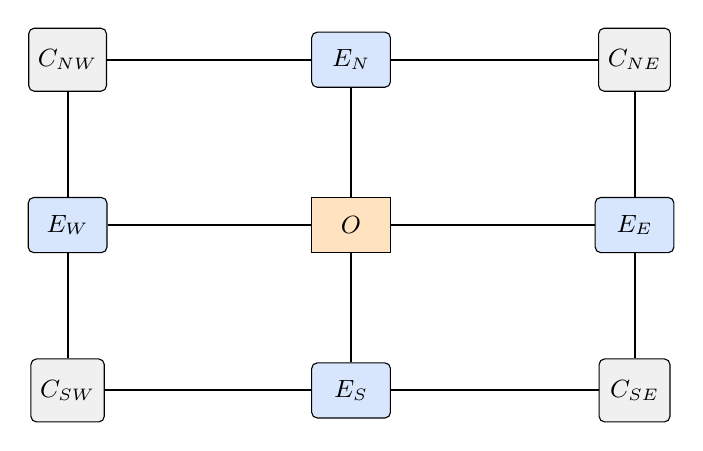
\begin{tikzpicture}[x=1.8cm,y=1.05cm]
\node[envcap] (nw) at (0,2) {$C_{NW}$};\node[r] (n) at (2,2) {$E_N$};\node[envcap] (ne) at (4,2) {$C_{NE}$};
\node[r] (w) at (0,0) {$E_W$};\node[o] (o) at (2,0) {$O$};\node[r] (e) at (4,0) {$E_E$};
\node[envcap] (sw) at (0,-2) {$C_{SW}$};\node[r] (s) at (2,-2) {$E_S$};\node[envcap] (se) at (4,-2) {$C_{SE}$};
\foreach \a/\b in {nw/n,n/ne,ne/e,e/se,se/s,s/sw,sw/w,w/nw,n/o,w/o,e/o,s/o}{\draw[wire] (\a)--(\b);}
\end{tikzpicture}
\caption{CTM 环境的实际八个未知张量。$O$ 是局域 PEPS 双层张量，不是额外的优化变量。}
\end{figure}

吸收相邻 edge 和局域网络，得到四个扩大角 $Q_i$；它们的切口空间含环境腿及新增 PEPS 腿。
在每个切口，把四角沿有向闭环收缩，得到线性算符 $M_i$。示意为
\[
Q_1\longrightarrow Q_2\longrightarrow Q_3\longrightarrow Q_4\longrightarrow Q_1.
\]
这里的闭环不能直接当作四个普通数组的乘积：\texttt{graded\_cycle\_v2.jl}
显式处理 dual、fusion 和 parity twist，包括环境 $\chi$ 腿；闭环用 matrix-unit 插入作过独立符号检查。

\textbf{投影如何得到？} 对每个 parity block 的 $M_i$ 和 $M_i^\dagger$ 分别做有序 Schur 分解，
选出匹配的右、左不变子空间基 $Z_R,Z_L$。保留完整模长群，并保持指定的 even/odd 秩；
无法恰好满足秩预算时拒绝该步，不静默减少 $\chi$。这个选择不一定等于简单的最大模前 $\chi$ 个根。
令
\[
Z_L^\dagger Z_R=U\Sigma V^\dagger,\qquad
R=Z_RV\Sigma^{-1/2},\quad L=\Sigma^{-1/2}U^\dagger Z_L^\dagger.
\]
于是 $LR=I$，$P=RL$ 是扩大切口上的斜投影，通常 $L\ne R^\dagger$。
检查 $M_iR=RK$、$LM_i=KL$、$P^2=P$、$[M_i,P]=0$。
交叉重叠病态或所选谱群无法分离时拒绝更新。
这一步的双正交化是\textbf{扩大角的保留子空间}双正交化，不是导出 MPS 后的整条链双正交规范。

\clearpage
\subsection{四个切口如何一起更新？}
四套投影都从同一轮冻结的环境计算。令 $P_i=R_iL_i$，相邻切口还必须满足
\[
P_iQ_i\simeq Q_iP_{i+1},\qquad i\pmod 4.
\]
这个 intertwiner 检查保证角两端选出的子空间相容。通过后才同时压缩扩大 corners 和 edges：
\[
C_i'=L_iQ_iR_{i+1},\qquad E_i'=L_{\rm out}\,\widehat E_i\,R_{\rm in}.
\]
最后两式表示端口对应的有向张量收缩；实现使用 \texttt{PL/PR} 的 fusion 形式，不能省略 graded 接线。
\begin{figure}[H]\centering
\begin{tikzpicture}[node distance=7mm]
\node[box,fill=rc,text width=11cm] (a) {四角、四边 $\mathcal C_n$};
\node[box,text width=11cm,below=of a] (b) {吸收网络：扩大角 $Q_i$、四个闭环 $M_i$};
\node[box,text width=11cm,below=of b] (c) {左右 Schur 子空间 $\rightarrow$ 交叉 SVD $\rightarrow$ 四套 $L_i,R_i$};
\node[box,text width=11cm,below=of c] (d) {检查秩、谱分离、双正交性、相邻切口 intertwiner};
\node[box,fill=oc,text width=11cm,below=of d] (e) {同时 renormalize 四角四边，得到 $\mathcal C_{n+1}$};
\node[box,fill=lc,text width=11cm,below=of e] (f) {导出边界，重新检查中心方程、关联函数和 bare/direct};
\foreach \a/\b in {a/b,b/c,c/d,d/e,e/f}{\draw[arr] (\a)--(\b);}
\end{tikzpicture}
\caption{实际 simultaneous 分支的一轮。局域投影代数通过，不等于外层环境已经驻定。}
\end{figure}

对应源码位于 \path{benchmark/eigctm/}：
\texttt{oblique\_whole\_schur.jl} 构造 $L,R$；
\texttt{whole\_clusters.jl} 选择完整模长群；
\texttt{simultaneous\_whole.jl} 检查四切口并调用
\texttt{PEPSKit.renormalize\_simultaneously}。
这不是完整 periodic-Schur 算法：当前逐切口求子空间，再检查相容性。

阻尼实验使用 $\mathcal C'=(1-\alpha)\mathcal C+\alpha F(\mathcal C)$，但一般非酉 gauge 下
直接插值张量坐标并不可靠。实验中已区分真正的一步映射阻尼与两个历史环境的插值；
不能以原始张量差小或投影误差小单独宣布收敛。

\clearpage
\subsection{Edge 怎样变成 boundary MPS？现在到底收敛了吗？}
\begin{figure}[H]\centering
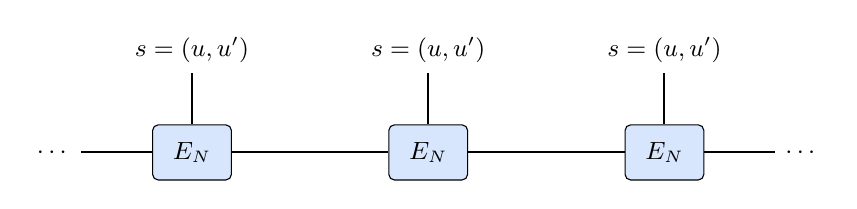
\begin{tikzpicture}[x=1.5cm]
\foreach \i in {0,2,4}{\node[r] (e\i) at (\i,0) {$E_N$};\draw[wire] (e\i.north)--++(0,.65) node[above] {$s=(u,u')$};}
\draw[wire] (e0)--(e2);\draw[wire] (e2)--(e4);
\draw[wire] (e0.west)--++(-.6,0) node[left] {$\cdots$};\draw[wire] (e4.east)--++(.6,0) node[right] {$\cdots$};
\end{tikzpicture}
\caption{重复 edge 的两条 $\chi$ 腿，把朝向 PEPS 的 $D^2$ 腿当作 MPS 局域指标。
这是半平面的候选边界波函数；corners 负责不同方向的连接，并未被当作每个 site 的中心。}
\end{figure}
代码 \texttt{boundary\_audit.jl} 实际执行
\[
R=\operatorname{InfiniteMPS}(E_N),\quad
S=\operatorname{InfiniteMPS}(E_S),\quad
L=\operatorname{InfiniteMPS}(\operatorname{spatial\_bra}(S_r)).
\]
$S_r$ 是南边界的右规范张量；空间 bra 映射保留费米腿方向与符号。
对整个 PEPS 和环境旋转一次，另取一组方向重复检查。因此并非只用一条 edge 代替四向环境。
导出后各自 canonical 化，再构造两条边界共同的中心算符。
熵测量仍使用 bare/direct，不改用 grown tail 或 endmap。

\textbf{截至本次文档整理（2026-09-22）的已核对历史记录：}
\begin{center}\small
\begin{tabular}{P{30mm}P{64mm}P{44mm}}
\toprule
候选 & 观察 & 判断\\\midrule
$\chi=16$ dense-Schur & 连续 135 步，$\xi_{\rm pair}$ 从 23.81 漂到 67.96，残差约 $10^{-3}$。 & 外层未驻定；不是立刻崩溃。\\
$\chi=16$ 真正一步阻尼 & 相邻切口误差约 $10^{-12}$，原中心方程误差仍约 $10^{-3}$。 & 投影准确，但未解决环境收敛。\\
$\chi=8$ CTM 种子加中心精修 & 两方向中心残差约 $5.45\times10^{-12}$、$3.28\times10^{-12}$；RDM 非 Hermitian，replica 相位失败。 & 中心求根成功，但不是可接受物理边界。\\
\bottomrule
\end{tabular}
\end{center}
最后一行不能算作 eigCTMRG 本身收敛：它额外运行了独立中心求解器。
两、三点 RDM 的非 Hermitian 范数分别约 $7.00\times10^{-4}$、$1.38\times10^{-3}$；
bare 的长度漂移很小也不能弥补相位错误。这些候选没有加入可信熵曲线。

\takeaway{结论：edge 到 boundary MPS 的转换已实现；大 $\chi$ 的稳定、物理正确的 eigCTMRG
环境尚未得到。不能笼统说所有尝试都只是“不收敛”：有外层漂移，也有后处理收敛到不通过物理检查的驻点。}
本节依据旧实验附册及对应源码整理，不代表本次重新运行数值任务或查询到了新的计算结果。
详细轨迹及作业编号见 \path{appendix_experiments_v18.tex} 的 CTM 初值与阻尼小节。

\end{document}
